\documentclass[10pt]{article}
\usepackage[a4paper,margin=0.4in]{geometry}
\usepackage[T1]{fontenc}
\usepackage[utf8]{inputenc}
\usepackage{lmodern}
\usepackage{microtype}
\usepackage{graphicx}
\usepackage{xcolor}
\usepackage{tabularx}
\usepackage{array}
\usepackage{booktabs}
\usepackage{titlesec}
\usepackage[hidelinks]{hyperref}

\definecolor{titleblue}{HTML}{163240}
\definecolor{accent}{HTML}{1D5A7B}
\definecolor{softgray}{HTML}{EEF3F6}

\setlength{\parindent}{0pt}
\setlength{\parskip}{1.5pt}
\setlength{\textfloatsep}{3pt}
\setlength{\floatsep}{3pt}
\setlength{\intextsep}{3pt}
\titleformat{\section}{\large\bfseries\color{titleblue}}{}{0em}{}[\titlerule]
\titlespacing*{\section}{0pt}{4pt}{2pt}
\pagestyle{empty}

\begin{document}

\begin{minipage}[t]{0.1\textwidth}

\includegraphics[width=0.88\linewidth]{slidev/logo.png}
\end{minipage}
\hfill
\begin{minipage}[t]{0.87\textwidth}
{\large\bfseries\color{titleblue} Route Decay Model Card} \\[-1pt]
{\small Huntrix Delta --- HackFusion 2026 \quad | \quad Logistic regression for 2-hour edge impassability prediction}
\end{minipage}

\vspace{0.15em}
\colorbox{softgray}{
\parbox{\dimexpr\textwidth-2\fboxsep\relax}{
\scriptsize \textbf{Summary:} The model predicts whether a route edge will become impassable within the next \textbf{2 hours}. Features are derived from the rainfall feed and edge context, then exported as JSON coefficients for both the Go backend and Expo mobile app.
}}

\section{Methodology Diagram}
\begin{center}
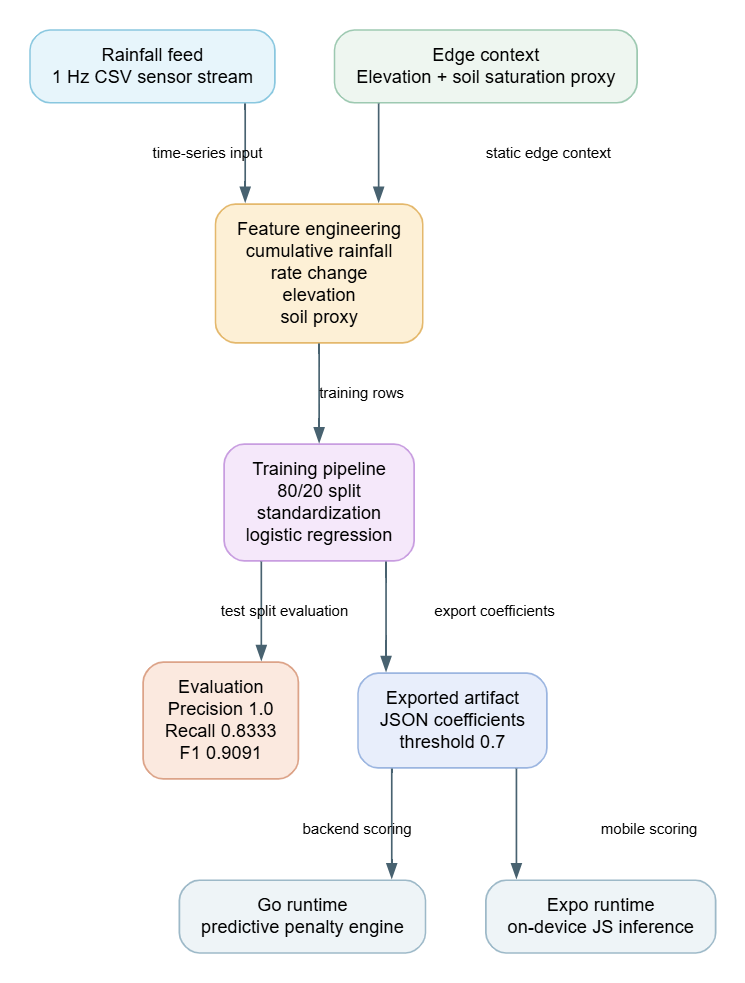
\includegraphics[width=0.7\textwidth]{model-card-methodology.png}
\end{center}

\section{Evaluation Results}
\scriptsize
\begin{tabular}{@{}lcccc@{}}
\toprule
Metric & Precision & Recall & F1 & Accuracy \\
\midrule
Value & 1.0 & 0.8333 & 0.9091 & 0.98 \\
\bottomrule
\end{tabular}

\vspace{0.2em}

\begin{tabular}{@{}lcccc@{}}
\toprule
Confusion Counts & TP & FP & TN & FN \\
\midrule
Value & 5 & 0 & 44 & 1 \\
\bottomrule
\end{tabular}
\small

\section{Notes}
\begin{itemize}\scriptsize
  \item Training split: \textbf{80/20}
  \item Threshold: \textbf{0.7}
  \item Features: \texttt{cumulative\_rainfall\_mm}, \texttt{rainfall\_rate\_change}, \texttt{elevation\_m}, \texttt{soil\_saturation\_proxy}
  \item Main limitation: labels are synthetic, so real-world confidence is lower than the demo metrics suggest.
\end{itemize}

\vspace{-0.2em}
{\scriptsize
\textbf{Primary artifacts:}
\texttt{ml/artifacts/route\_decay\_model.json},
\texttt{ml/artifacts/route\_decay\_metrics.json},
\texttt{docs/model-card.md}
}

\end{document}
